%% Explain the scenario created; how and when the agents are dropped;

The original work presented by \textit{Schwarzrock et al.}~\citep{MAS07} was based on a static context. In that scenario, important elements such as the tasks that compose the mission, or the number and the type of agents, are defined in the beginning and do not change during the mission execution.

However, as already mentioned, considering a military operation environment, this assumption is not realistic, limiting the usefulness of the solution in the real world. To explore a more realistic context, dynamism in the scenario must be considered. This work targets this aspect by considering a varying number of agents during the execution of the algorithms, randomly taking down of some agents. 
The agents removal follows a time slice $\mu$ defined by Eq. \ref{eq:uavs}, i.e., one UAV will be taken down in each interval defined by the total mission time (measured in ticks) divided by the initial number of agents in the team. This proceeds until a single UAV remains in the team, as shown by Algorithm \ref{algo:down}. This algorithm is implemented into the main loop of each original code variant proposed by~\citep{MAS07}, where the token exchange among agents occurs, as well as the task allocation, and it is executed in each pass of the main method.

\begin{equation} \label{eq:uavs}
	\mu = \frac{total\_time}{total\_agents}
\end{equation}

% Obs Prof Vander - verificar se nao é o caso de deixar o algoritmo com um formalismo mais matematico 
\begin{algorithm}[!ht]
	\caption{Pseudocode for taking down an UAV(agent) that is inserted after line \ref{line:AL_ini} of Alghorithm \ref{algo:swarm-gap} and used by the three variants proposed by the original study \citep{MAS07}}
	\label{algo:down}
	
	\SetAlgoLined
	\DontPrintSemicolon
	\SetKwBlock{Loop}{loop}{end loop}
	\SetKwFor{ForAll}{for all}{do}{end for}
	\SetNlSty{text}{}{:}
	\SetNlSkip{0.3em}
	
	t = current time in ticks \;
	\If {number of operational agents $>$ 1}{
	\If {($t \bmod \mu$) = 0 }{
	    Choose an agent randomly from those with resources \;
	    Remove all resources from the selected agent \;
	    Remove unfinished tasks from the selected agent \;
	    Operational agents counter is decreased by 1 \;
	    Update not visited agents list in the token\;
	    Set agent color as "red" \;
    	}
    	Increment time by 1 tick \;
	}
	
\end{algorithm}

A screen of the dynamic scenario running can be seen in Figure \ref{fig:screen01}. It illustrates the simulation graphical interface, where the symbol for the tasks is represented by a $X$ shape and the symbol for a \uav\ has the shape of an airplane. The black airplane represents a functional airplane and the red one represents a UAV dropped and out of operation.

\begin{figure}[h!]
	\begin{center}
		\fbox{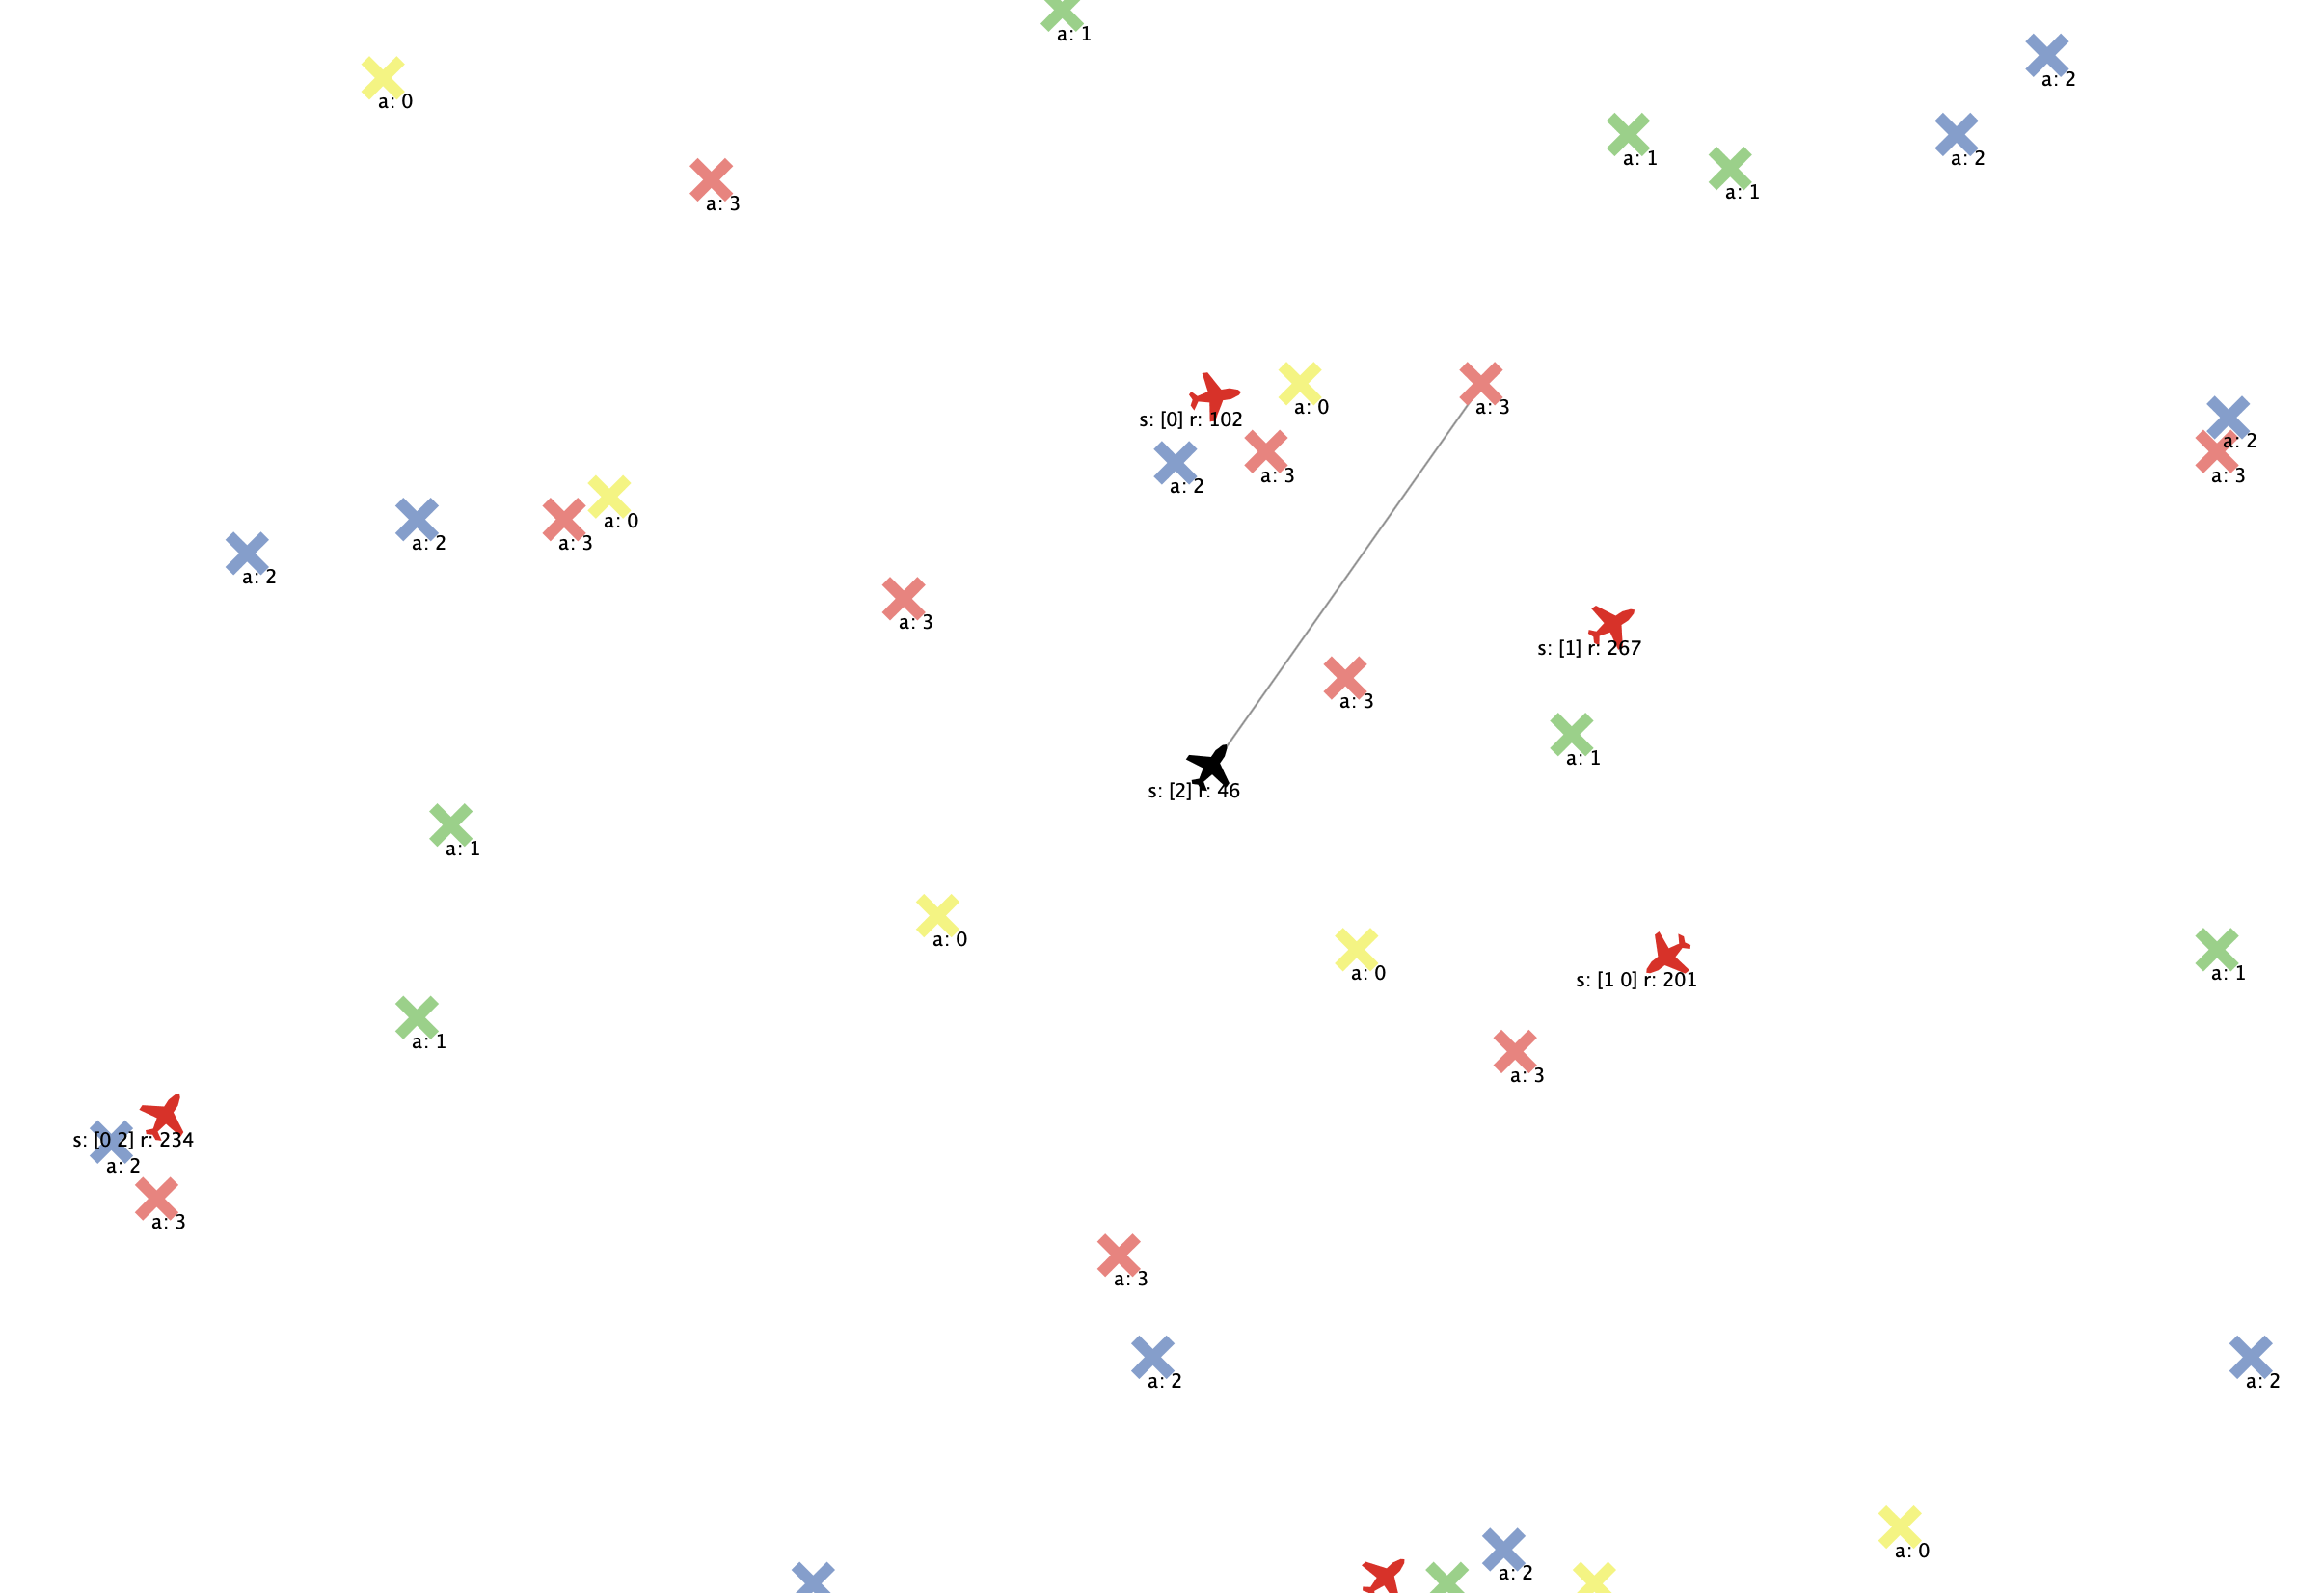
\includegraphics[scale=0.3]{fig/tela01.png}}
		\caption{NetLogo 5.3.1 screen with dropped UAVs in red, in the dynamic scenario}
		\label{fig:screen01}
	\end{center}
\end{figure}

As the quantity of agents changes during the execution, this characteristic gives dynamism to the context. It grants the capacity to analyze the agents' response and to assess the original algorithms in this new dynamic scenario. 

Furthermore, to reduce the standard deviation in the results, all experiments were executed 100 times instead of only 30, as it was done in the original study. It was noticed a decrease in the error using this increased number of runs.